\chapter{Cottontail DB}
\label{chapter:cottontaildb}

\emph{Cottontail DB}~\cite{Gasser:2020cottontail} is our reference implementation for the query, cost and index-models described in \Cref{chapter:system_model}. Starting out as a drop-in replacement for ADAMpro \cite{Giangreco:2016adam}, it has grown to be a full fledged \acrshort{dbms} with support for both classical boolean retrieval as well as proximity based search. Both aspects have been combined in a unified query and execution model and many explicit and implicit decisions, which are described in this chapter, went into its design.

\emph{Cottontail DB} is written in Kotlin\footnote{See: https://kotlinlang.org/} and runs on the \acrfull{jvm}. While an unorthodox choice of language and environment for a database, there are several prominent examples that were built for the \acrshort{jvm}, including but not limited to H2\footnote{See: https://www.h2database.com/}, HSQLDB\footnote{See: https://hsqldb.org/} or Derby\footnote{See: https://db.apache.org/derby/}. \emph{Cottontail DB}'s source code can be downloaded from GitHub\footnote{See: https://github.com/vitrivr/cottontaildb}. It is freely available under a permissive open source license and can be used as standalone application, Docker container or in an embedded mode.

\section{Data Model and Nomenclature} 

\emph{Cottontail DB} uses a data model very similar to that of other relational \acrshort{dbms}': All data is organized into \emph{entities} -- which correspond to tables or relations -- that consist of individual, strongly typed \emph{columns}. The different data types currently supported are listed in \Cref{table:cottontail_types}. Columns can hold values of the declared type or \texttt{NULL} to indicate the absence of information (if the column has been declared as being nullable). 

An entity can then host multiple \emph{records}, which correspond to rows or tuples in the table. Since \emph{Cottontail DB} is a column store, records are only logical constructs in memory and do not correspond to the physical data representation on disk. Consequently, records are assembled on-the-fly as queries are being executed. As with columns, every record is also strongly typed, wherein a record is a tuple type of its strongly typed elements. Internally, every record is uniquely identified by a \emph{tuple ID}, which is a \texttt{long} value that can be used to address the record within an entity or a (in-memory) \emph{recordset}. This tuple ID is not exposed to the outside because it remains at the discretion of the storage and execution engine to generate, assign, change and (re-)use them as data gets re-organized.

Furthermore, \emph{Cottontail DB} allows for multiple entities to be grouped into \emph{schemata}, which currently serves an organisational purpose only. Every entity can also host one or multiple secondary \emph{indexes} that index a single or multiple \emph{columns} for more efficient data access.

To address database objects, \emph{Cottontail DB} uses a hierarchical namespace, i.e., every schema, entity, column and index must be uniquely named by a \emph{fully qualified name}. All the information about the database objects is tracked in an internal \emph{catalogue}, which is backed by the main storage engine.

\begin{table}

    \caption{Data types supported by \emph{Cottontail DB}. Types in the numeric, vector and complex domain allow for domain specific arithmetics.}
    \label{table:cottontail_types}

    \begin{tabular}{| l || c | c | c | l |}
        \hline
        \textbf{Name} & \textbf{Numeric} & \textbf{Vector} & \textbf{Complex} & \textbf{JDBC / SQL}\\ 
        \hline
        \hline
        String & & & & \texttt{VARCHAR} \\ 
        \hline
        Date & & & & \texttt{TIMESTAMP}\\
        \hline 
        Boolean & \checkmark & & & \texttt{BOOLEAN} \\ 
        \hline
        Byte & \checkmark &  & & \texttt{TINYINT} \\ 
        \hline
        Short & \checkmark &  & & \texttt{SMALLINT} \\ 
        \hline
        Int & \checkmark &  & & \texttt{INT}\\ 
        \hline
        Long & \checkmark &  & & \texttt{BIGINT}\\ 
        \hline
        Float & \checkmark &  & & \texttt{REAL}\\ 
        \hline
        Double & \checkmark &  & & \texttt{DOUBLE}\\ 
        \hline
        Complex 32 & \checkmark &  & \checkmark & - \\ 
        \hline
        Complex 64 & \checkmark &  & \checkmark & - \\ 
        \hline
        Boolean Vector & \checkmark & \checkmark & & \texttt{ARRAY[BOOLEAN](1, d)} \\ 
        \hline
        Integer Vector & \checkmark & \checkmark & & \texttt{ARRAY[INT](1, d)} \\ 
        \hline
        Long Vector & \checkmark & \checkmark & & \texttt{ARRAY[BIGINT](1, d)}\\ 
        \hline
        Float Vector & \checkmark & \checkmark & & \texttt{ARRAY[REAL](1, d)}\\ 
        \hline
        Double Vector & \checkmark & \checkmark & & \texttt{ARRAY[DOUBLE](1, d)}\\ 
        \hline
        Complex32 Vector & \checkmark & \checkmark & \checkmark & - \\ 
        \hline
        Complex32 Vector & \checkmark & \checkmark & \checkmark & - \\ 
        \hline
    \end{tabular}
    
\end{table}
\section{Architecture} 

The main components of \emph{Cottontail DB} are depicted in \Cref{figure:cottontail_architecture}. We use the path a query takes within the system, as indicated by the directed arrows, to illustrate the components involved in its execution.

At a high level, every query must undergo \emph{parsing}, \emph{binding}, \emph{planning} and \emph{execution} in that order. However, planning can be skipped for certain types of queries, such as, \acrshort{ddl} or some \acrshort{dml} statements. We will describe the aforementioned steps in reverse order in the following sections, since important concepts can be introduced more naturally that way.

\begin{figure}[bt]
    \centering
    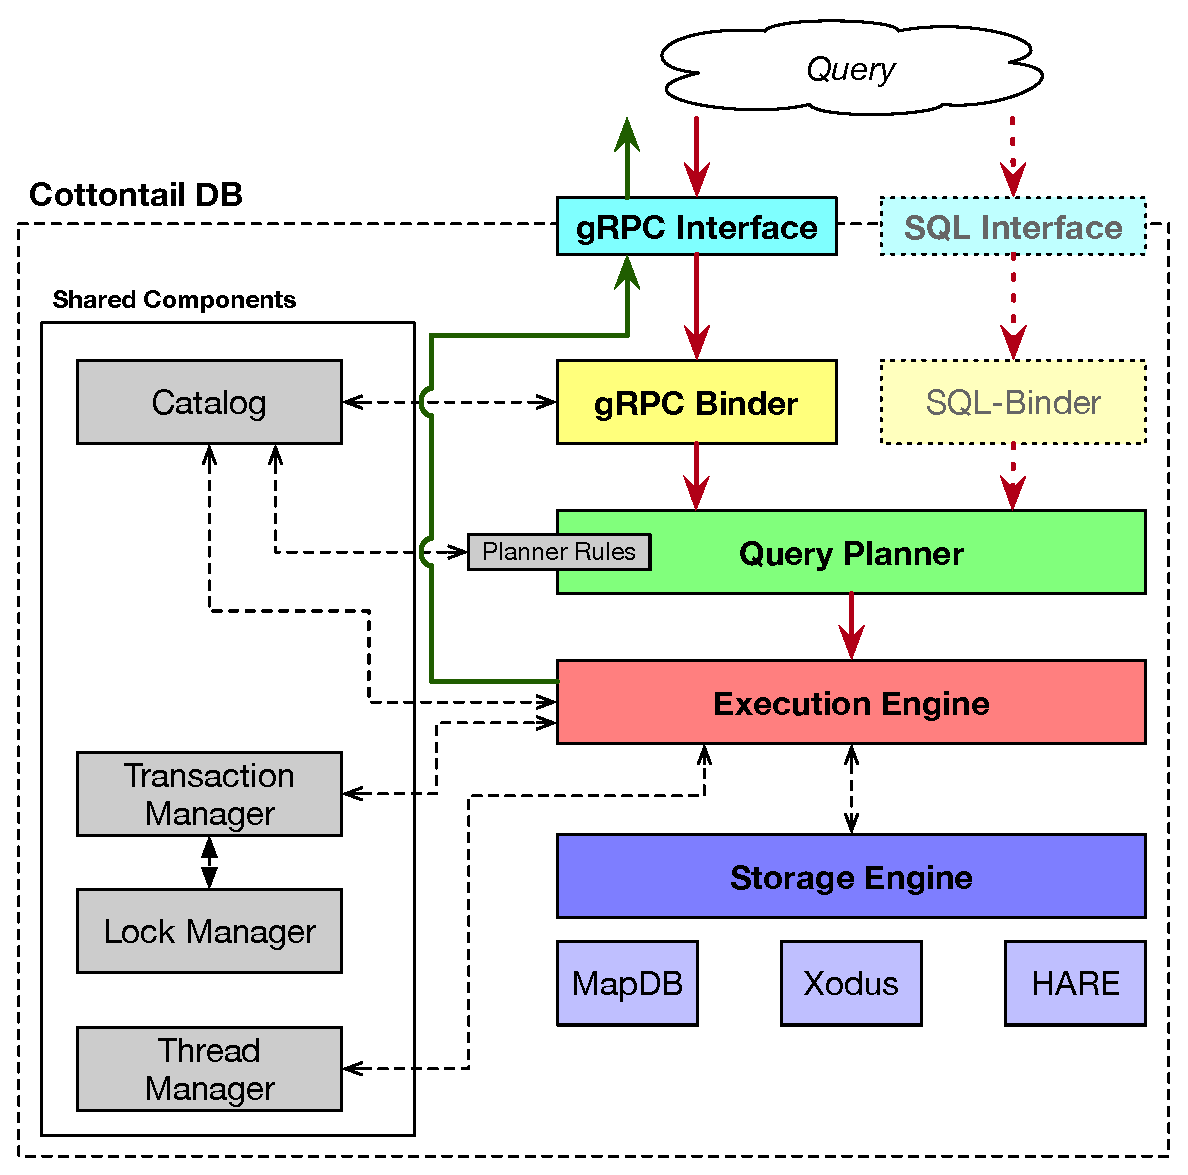
\includegraphics[width=\textwidth]{figures/architecture.eps}
    \caption{Architecture diagram of Cottontail DB's main components. The directed arrows indicate the path a query takes within the system. The dashed, double arrows indicate interactions between components.}
    \label{figure:cottontail_architecture}
\end{figure}


\subsection{Query Implementation and Execution}

\emph{Cottontail DB} implements an \emph{iterator model} for query execution. This means that an implemented query is a pipeline of operators, wherein each operator processes single records it receives from its upstream input operator(s) and passes single records to the next operator in the pipeline. Conceptually, \emph{Cottontail DB} distinguishes between \emph{Nullary}, \emph{Unary}, \emph{Binary} and \emph{N-Ary} operators, which differ in the number of inputs they can accept (0, 1, 2 or N). Furthermore, some operators require materialization of intermediate resultsets and therefore act as pipeline breakers since they must collect all inbound records before they can start handing them down (e.g., sort operators). The most important types of operators implemented by \emph{Cottontail DB} along with their correspondence to the relational operators described in Chapters \ref{chapter:theory_databases} and \ref{chapter:system_model} are listed in \Cref{table:cottontail_operators}.

\begin{table}
    \caption{Main types of operators implemented by \emph{Cottontail DB} alongside with their arity, their correspondence to relational operators and whether or not they require materialization.}
    \label{table:cottontail_operators}

    \begin{tabular}{| l || c | p{20mm}  | c | p{75mm} |}
        \hline
        \textbf{Type} & \textbf{Arity} & \textbf{Rel. Op.} & \textbf{Mat.} & \textbf{Description} \\ 
        \hline
        \hline
        Scan & 0 & $\projection_{\chi}$ \newline $\selection_{\mathcal{P}}$ \newline $\rho_{\attribute_\mathtt{A} \rightarrow \attribute_\mathtt{B}}$ & & Act as data sources. Usually scan an \emph{entity} or an \emph{index} and thus interact directly with the storage engine. \\ 
        \hline
        Fetch & 1 & $\projection_{\chi}$ & & Extend every incoming record by fetching one or multiple columns and appending them to the record. Usually interact directly with the storage engine to perform random reads. \\
        \hline 
        Function & 1 & $\projection_{\chi}$ & & Extend every incoming record by evaluating a specific function and appending the result as a new column to the record.\\ 
        \hline
        Filter & 1 & $\selection_{\mathcal{P}}$ & & Filter incoming records by evaluating a given predicate. Records that don't match the predicate are not handed down the pipeline. \\ 
        \hline
        Sort & 1 & $\tau_{(\mathcal{A},\uparrow\downarrow)}$ & \checkmark & Sort the incoming records based on the specified columns in the specified direction. \\ 
        \hline
        Limit & 1 & $\lambda_k$ & &  Skip and drop incoming records according to specification and thus limit the number of out-bound records to a specified number \\ 
        \hline
        Project & 1 & $\projection_{\chi}$ \newline $\rho_{\attribute_\mathtt{A} \rightarrow \attribute_\mathtt{B}}$ & & A terminal operator that actively removes and/or renames columns in the incoming records. This is sometimes necessary because columns may be fetched for processing but are not desired in the final result. \\ 
        \hline
        \hline
    \end{tabular}  
\end{table}

Every operator is implemented in Kotlin and pre-compiled to byte code. Ergo, there is no on-the-fly code generation during runtime. The operator implementations are derived from the plan that is selected in the planning stage.

\subsubsection{Execution Model}

Operators in \emph{Cottontail DB} are implemented as \emph{coroutines}, i.e., every operator is a suspendable function that yields to the next operator in the pipeline upon emission of a value. Each operator collects a single record from its input operator(s), performs processing and forwards the resulting record by calling \texttt{emit()}, thus yielding to the next operator in the pipeline. Source operators usually iterate some data collection through a cursor and thus only \texttt{emit()} values, whereas sink operators \texttt{collect()} values without emiting anything (practically, the collected values are usually sent to the client that issued the query). Pipeline breaking operators are required to \texttt{collect()} all inbound values before they can start to \texttt{emit()}, i.e., they materialize a recordset. The suspension and continuation of function calls is orchestrated by Kotlin's coroutines ``Flow'' framework\footnote{See: https://kotlinlang.org/docs/coroutines-overview.html}. A very simple example of a naive operator pipeline is provided in \Cref{figure:cottontail_execution_model_simple}.

\begin{figure}[bt]
    \centering
    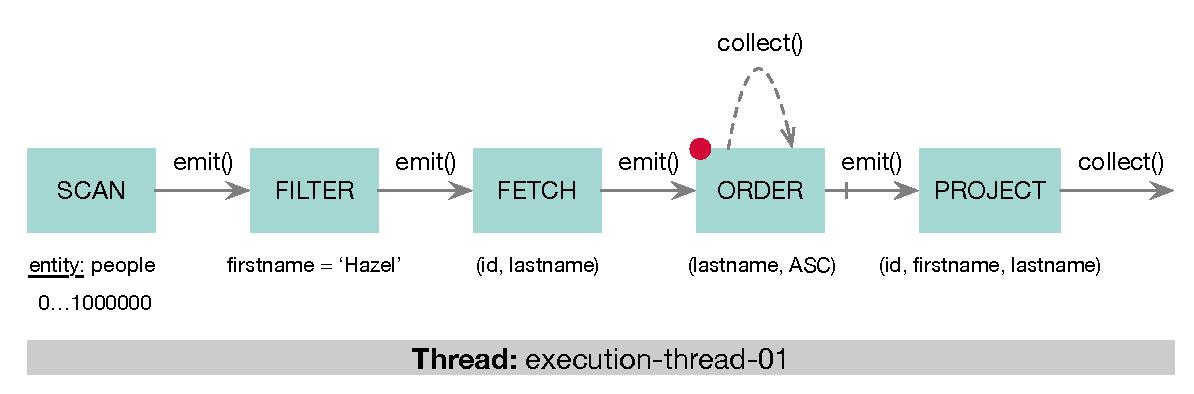
\includegraphics[width=0.9\textwidth]{figures/execution-model-simple}
    \caption{Operator pipeline for a boolean query that filters the entity \emph{people} for entries with the \emph{firstname} ``Hazel'' and sorts the output by column \emph{lastname}. Pipeline breaking operators are indicated by the red dot.}
    \label{figure:cottontail_execution_model_simple}
\end{figure}

Inter-query parallelism is achieved, by collecting different operator pipelines on different threads. The assignment of operator pipeline to thread is delegated to a \emph{dispatcher}, which has a defined thread pool at its disposal and which is part of Kotlin's coroutines framework. 

However, this execution model also allows for intra-query parallelism, which is used for queries that incur high CPU cost. This is realised in a \emph{data parallel} fashion by partitioning on the input. The decision whether or not to allow for parallelism is made upon implementation of a query -- i.e., the last step after the final plan has been selected -- since it requires structural changes to the operator pipeline. The degree of parallelism depends on the expected CPU cost of the plan and the available CPUs on the machine \emph{Cottontail DB} is running on.

To prepare for intra-query parallelism, part of the operator pipeline is partitioned wherein every partition operates on a fraction of the input data. Since not all steps in a pipeline can be parallelised effectively, usually only parts of the pipeline are partitioned. Whether parallelisation is possible at a given point in the pipeline depends on whether the operator itself as well as all upstream operators allow for parallelisation, which is queried upon implementation. An additional \emph{merge} operator is introduced after such an operator, which synchronizes and merges all the incoming strands using a \acrshort{fifo} scheme. Therefore, sort operations must take place after a merge, since any order established before the merge will be lost. An example for this is given in \Cref{figure:cottontail_execution_model_parallel}.

\begin{figure}[bt]
    \centering
    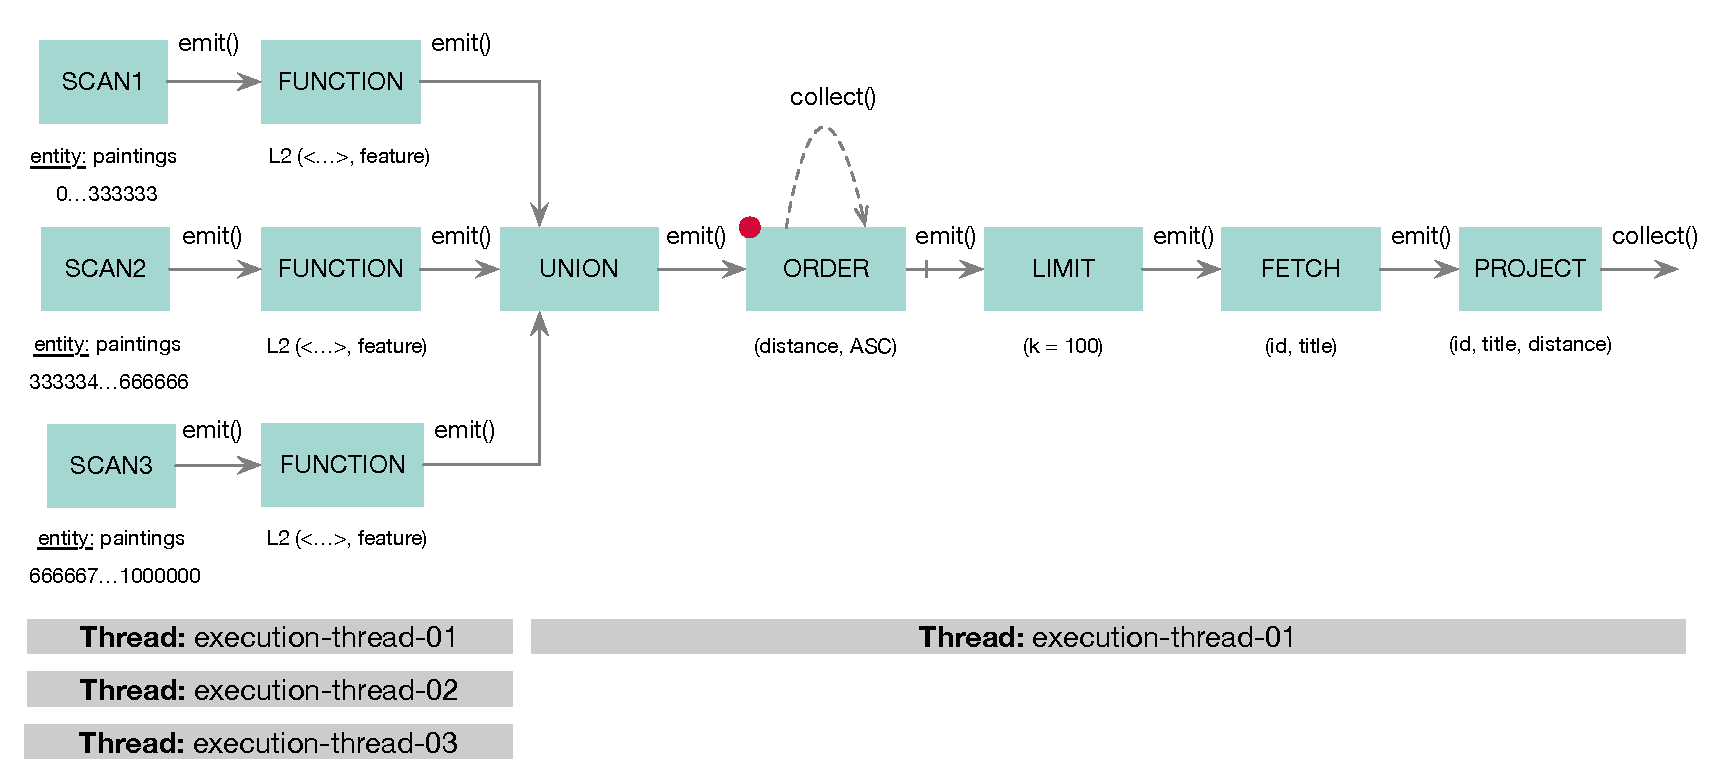
\includegraphics[width=0.9\textwidth]{figures/execution-model-parallel}
    \caption{Operator pipeline for a boolean query that filters the entity \emph{people} for entries with the firstname ``Hazel'' and sorts the output by column \emph{people}. The \emph{scan} and \emph{filter} steps are partitioned and merged before fetching, sorting and projecting takes place, which allows for parallelsm.}
    \label{figure:cottontail_execution_model_parallel}
\end{figure}

With an operation pipeline prepared in this fashion, it again remains up to the dispatcher to allocate parts of the pipeline to concrete threads. \emph{Cottontail DB} only declares how allocation should take place by chosing the appropriate type of dispatcher. Consequently, the level of partitioning is merely an upper bound on parallelism without any guarantee, that every strand will be processed by a dedicated thread. 

\subsection{Query Planner}

The goal of \emph{query planning} is to find a cost-optimal execution plan for a query given any \emph{policy} valid for the current query context and \emph{Cottontail DB}'s cost model. The input into the query planner a logical representation of the operators that should be executed as part of the operator pipeline, which we call the \emph{canonical operator node tree}. It results directly from the \emph{query binding} stage.

Query planning in \emph{Cottontail DB} takes place in three steps: First, and optionally, the canonical operator node tree is compared to the \emph{plan cache}. If the cache contains a hit for that tree, the already optimized plan in the cache can be re-used and all the subsequent steps can be skipped. Second, if there is no hit in the cache or the cache is bypassed, the canonical operator node tree undergoes \emph{optimization}. The optimization step generates different versions of the input plan by applying optimization rules that act on and manipulate the tree to generate new, equivalent plans. Finally, once optimization has concluded, the plan that minimizes the expected cost is selected and \emph{implemented}, that is, converted to a concrete sequence of executable operators.

\subsubsection{Basic Optimization Algorithm}

The query planner used by \emph{Cottontail DB} is rather naive and can be categorized as a rule-based query planner\todo{Find reference on Volcano Planner paper.}. As the name implies, it generates new plans by enumerating and applying a set of rules to the input plan(s) in a recursive fashion. These rules are transformations that recognize patterns in the structure of the (canoncial) operator node tree and try to re-arange and/or replace nodes in the tree to generate a more optimal but equivalent version of the plan.

The optimization follows the same, basic algorithm: The available list of rules is enumerated and every rule is applied to every node starting from the base of the tree. The application of rules takes place recursively, i.e., every node propagates a rule up the tree to its inputs. At every node, the rule first checks if it can be applied to the current node. This check usually incurs little cost and simply considers the type of node and other, available properties. If the check is successful, the actual application of the rule follows. This application may or may not yield a new version of the query plan, depending on more complex and more costly factors, such as the availability of an index, which requires a catalogue lookup. If a new plan results from the application of a rule, that new query plan is stored in a \emph{memoization table} along with the input plan for future reference. 

Every planning stage involves a defined number of passes, and the sum of all plans generated by one pass act as the input for the next. All the intermediate plans are therefore run through the same algorithm and all the rules are applied again. Consequently, the search space grows exponentially with the complexity of the input plan, the number of rules to apply and the number of passes. To address this, \emph{Cottontail DB}'s query planner employs certain heuristics to keep the search space manageable:

\begin{itemize}
    \item Very large, complex plans (e.g., stemming from sub-selects or JOINs) are broken into groups and every group is optimized and treated as an isolated plan. The assumption being that the combination of smaller, near-optimal plans must be close to optimal as well.
    \item The planning of every group is done in two stages -- a \emph{logical} and \emph{physical} stage -- with distinct and disjoint sets of rules. The results of the logical stage act as an input for the physical stage.
    \item Logical and physical query plans are uniquely identified by a hash. Memoization in combination with the aforementioned hash is used to track trees that have already been optimized and skip them.
    \item Physical execution plans generated in the second stage are actively pruned by the planner between the different passes based on the cost estimate for the plan.
\end{itemize}

Between the logical and the physical planning, there is a step that maps every logical operator node to its naive, physical counterpart. The number of passes per stage and active pruning of plans during the physical phase are used to steer the high-level behaviour of the query planner. During the logical phase, the goal is to generate as many, equivalent, logical query representations as possible to have a corpus of plans to optimize on (expansion phase). In contrast, during the physical phase, the planner tries to limit the number of intermediate plans to prevent the search space from exploding.

\subsubsection{Plan Caching}

The plan cache is an optimization mechanism that amortizes the cost of the potentially expensive query planning if a certain type of query is encountered multiple times. At its core, the cache maps the hash code of every incoming canonical operator tree to the resulting, optimized physical plan. If the same query is encountered again, that plan can be looked-up and re-used directly, hence, avoiding another round of planning.

Currently, there are certain limitations to the plan cache mechanism in \emph{Cottontail DB}, which is why it is disabled by default. Firstly, the actual execution performance of a plan is not being evaluated against the cost model, i.e., the level of optimality of an execution plan is not assessed. And secondly, there is no mechanism that invalidates cached entries as changes to the data occur. 

\subsubsection{Logical Optimization}

The logical optimization step acts on structural properties of the operator node tree and aims at expanding the list of query plans in a way that increases the chance of finding the optimal plan during the physical phase. The logical optimization stage currently involves the following type of rules:

\begin{description}
    \item[Defer Fetch On Scan Rewrite Rule] This rules tries to defer access to columns upon scanning the data. It makes sure, that only columns are accessed during a table scan, that are required by the first operator following the scan that requires the presence of specific columns. All remaining columns are pushed down in the tree into a dedicated \emph{fetch} operation following that node.
 
    \item[Defer Fetch On Fetch Rewrite Rule] This rule tries to defer access to columns upon fetching data. Similarly to the \emph{Defer Fetch on Scan Rewrite Rule}, it pushes the fetching of columns not required by any of the downstream operators that express a specific requirement, into a dedicated fetch operation following such an operator.
    
    \item[Conjunction Rewrite Rule] This rule refactors a filter operator evaluating a conjunctive predicate into two consecutive \emph{filter} operators, one for each side of the conjunction. There are two versions of this rule, one that applies the left side first and one that applies the right side first.
\end{description}

The first two rules make sure, that columns are accessed only if they are needed and as close to the site of processing as possible. Furthermore, and since these rules are applied multiple times, columns that are not accessed at all will eventually be pushed out and eliminated from the tree completely. This is illustrated in the example given in \Cref{figure:cottontail_logical_rule_fetch}. Since Cottontail DB is a column store, deferal of column access can drastically reduce I/O, especially in the presence of filtering predicates or if a column is not needed. 

\begin{figure}[bt]
    \centering
    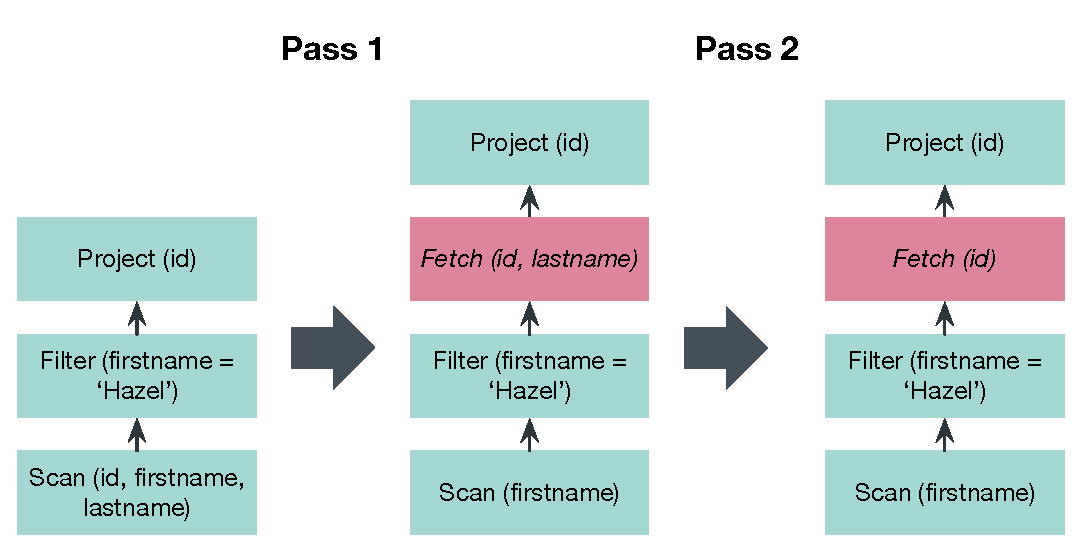
\includegraphics[width=0.9\textwidth]{figures/logical-rule-fetch}
    \caption{Illustration of deferal of column access. In the first pass, access to columns \emph{id} and \emph{lastname} is defered until after the filter operation, because the filter only requires \emph{firstname}. In the second pass, access to \emph{lastname} is eliminated completely.}
    \label{figure:cottontail_logical_rule_fetch}
\end{figure}

The conjunction rewrite rule decomposes filtering predicates that contain conjuctions. This is illustrated in the example given in \Cref{figure:cottontail_logical_rule_conjunction}. The applicaton of this rule can be seen as a preparation for the physical optimization phase, where specific predicates may be pushed down to a secondary index.

\begin{figure}[bt]
    \centering
    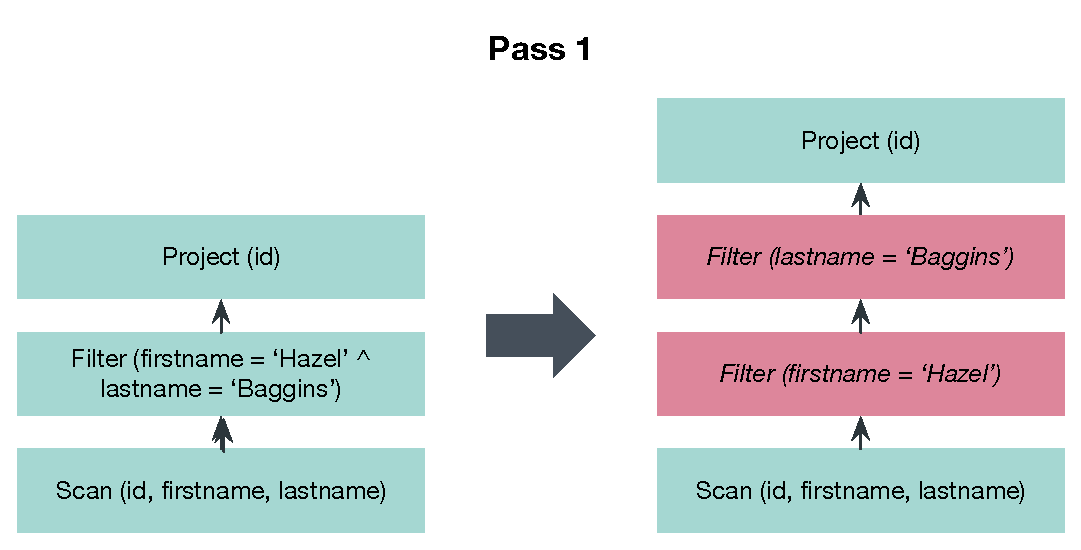
\includegraphics[width=0.9\textwidth]{figures/logical-rule-conjunction}
    \caption{Illustration of decomposing conjunctive predicates. In this example, the filter on the column \emph{firstname} may be pushed down to an index during physical optimization, if such an index is available.}
    \label{figure:cottontail_logical_rule_conjunction}
\end{figure}

\subsubsection{Physical Optimization}

The physical optimization step tries different implementations of operators to arrive at a more cost-effective plan. While structural changes to the operator tree may be possible, the focus lies on implementation aspects.  At a high level, we distinguish between the following three types of rules:

\begin{description}
    \item[Predicate Pushdown Rules] These rules try to push down \emph{filter} predicates or \emph{function} invocations to the \emph{scan} operation, usually by leveraging a secondary index. For example, an entity scan followed by a filter can be replaced by a more efficient scan of a $B^+$-index followed by a \emph{fetch} operation or nearest neighbor search operation can be delegated to a high-dimensional index.
 
    \item[Summarization Rules] These rules try merge operations to arrive at a more efficient execution. For example, a \emph{sort} operation followed by a \emph{limit} operation can be replaced by a single, \emph{limiting heap sort} operation, which applies sorting and limiting in a single step. Combining these two operations and the use of the heap-sort algorithm allows for more effective sorting in terms of CPU and memory cost, as compared to naively sorting all records first and then limiting to the top $k$ records after.
    
    \item[Implementation Rules] These rules simply replace different implementations of a operation one-to-one, e.g., hash-join vs. nested-loop join for a theoretical JOIN operation.
\end{description}

After each pass in the physical optimization step, the list of resulting plans is pruned to the $n$ best performing plans before handing them to the next pass. By this, we limit the size of the search space that is being explored. Once all passes have concluded, the best plan in terms of cost is selected and implemented.

\subsection{Query Parsing and Binding}
As every \acrshort{dbms}, \emph{Cottontail DB} uses a query language that allows for interaction with other systems. These interactions include data definition, data management, transaction management and the formulation of queries. In its current version, \emph{Cottontail DB} uses a query language based on \emph{gRPC}\footnote{See: https://grpc.io/}, hence, all queries are expressed as \emph{Protocol Buffer}\footnote{See: https://developers.google.com/protocol-buffers/} messages. Internally, the gRPC endpoint is a collection of four services for handling \acrshort{ddl}, \acrshort{dml}, \acrshort{dql} and transaction management messages. The parsing of incoming messages, the mapping of messages to the correct service and endpoint and low-level handling of communication with clients is delegated to the gRPC Kotlin library. 

The reason for the choice of gRPC is threefold: Firstly, Cottontail DB's predecessor -- ADAMpro -- already used and introduced gRPC into the \emph{vitrivr} stack. Consequently, building on this work greatly simplified the task of integrating \emph{Cottontail DB}. Secondly, gRPC -- being a platform independent remote procedure call framework -- introduces out-of-the-box support for a large range of programming environments\footnote{Furthermore, there are specialized client libraries for Java, Kotlin and Python}. And finally, the gRPC Kotlin library greatly simplified the task of structuring query endpoints, parsing incoming query messages and handling the query responses.

Irrespective of the use of gRPC, Cottontail DB is compatible with the SQL standard insofar as it supports a specific feature. This was shown by be the successful integration of \emph{Cottontail DB} as a storage engine for \emph{Polypheny DB} \todo{Ref: Polypheny DB + joint publication}. Consequently, it is possible to add additional endpoints that can accept, for example, \acrshort{sql} queries. However, for complete SQL compliance, one would have to add language features that are currently not supported by \emph{Cottontaild DB} (e.g., JOINS). Furthermore, handling the technical details of parsing the incoming query and communication with the client must be handled as well, which leads to the implementation of many different standards such as \acrshort{jdbc} or \acrshort{odbc}.

Irrespective of its source, any incoming query message undergoes a \emph{binding} step in \emph{Cottontail DB}. Query binding includes three aspects:

\begin{enumerate}
    \item Names that reference database objects such as entities, columns and indexes are resolved using \emph{Cottontail DB}s catalogue and replaced by concrete pointers to the respective object.
    \item Literal values, e.g., in predicates, are extracted and cached for late binding. This allows for reuse of execution plans with different values.
    \item The parsed message is converted into a \emph{canonical operator node tree} that logically represents the query.
\end{enumerate}

The result of the parsing and binding step is the canonical operator node tree, which acts as a logical and unoptimized query representation.  Every node in the tree represents an operator that acts on a \emph{record} or \emph{tuple} and that must be executed in order to generate the result specified by the query. The conversion of a message to a tree is performed in a naive manner and only syntactic checks and optimization are performed at this stage (e.g., type checks, removal of trivial predicates such as ``$1 = 1$'').

\subsection{Storage}
\subsubsection{MapDB}
\subsubsection{Xodus}
\subsubsection{HARE}



\section{Additional Functionality}

\todo[inline]{Implementation chapter for Cottontail DB}